\documentclass[../main.tex]{subfiles}

\begin{document}

\chapter{Diffusion models for cell wall permeability}
\label{cha:diffusion}

\section{Methods}
\label{sec:diffmodelling}

\begin{figure}[ht]
  \centering
  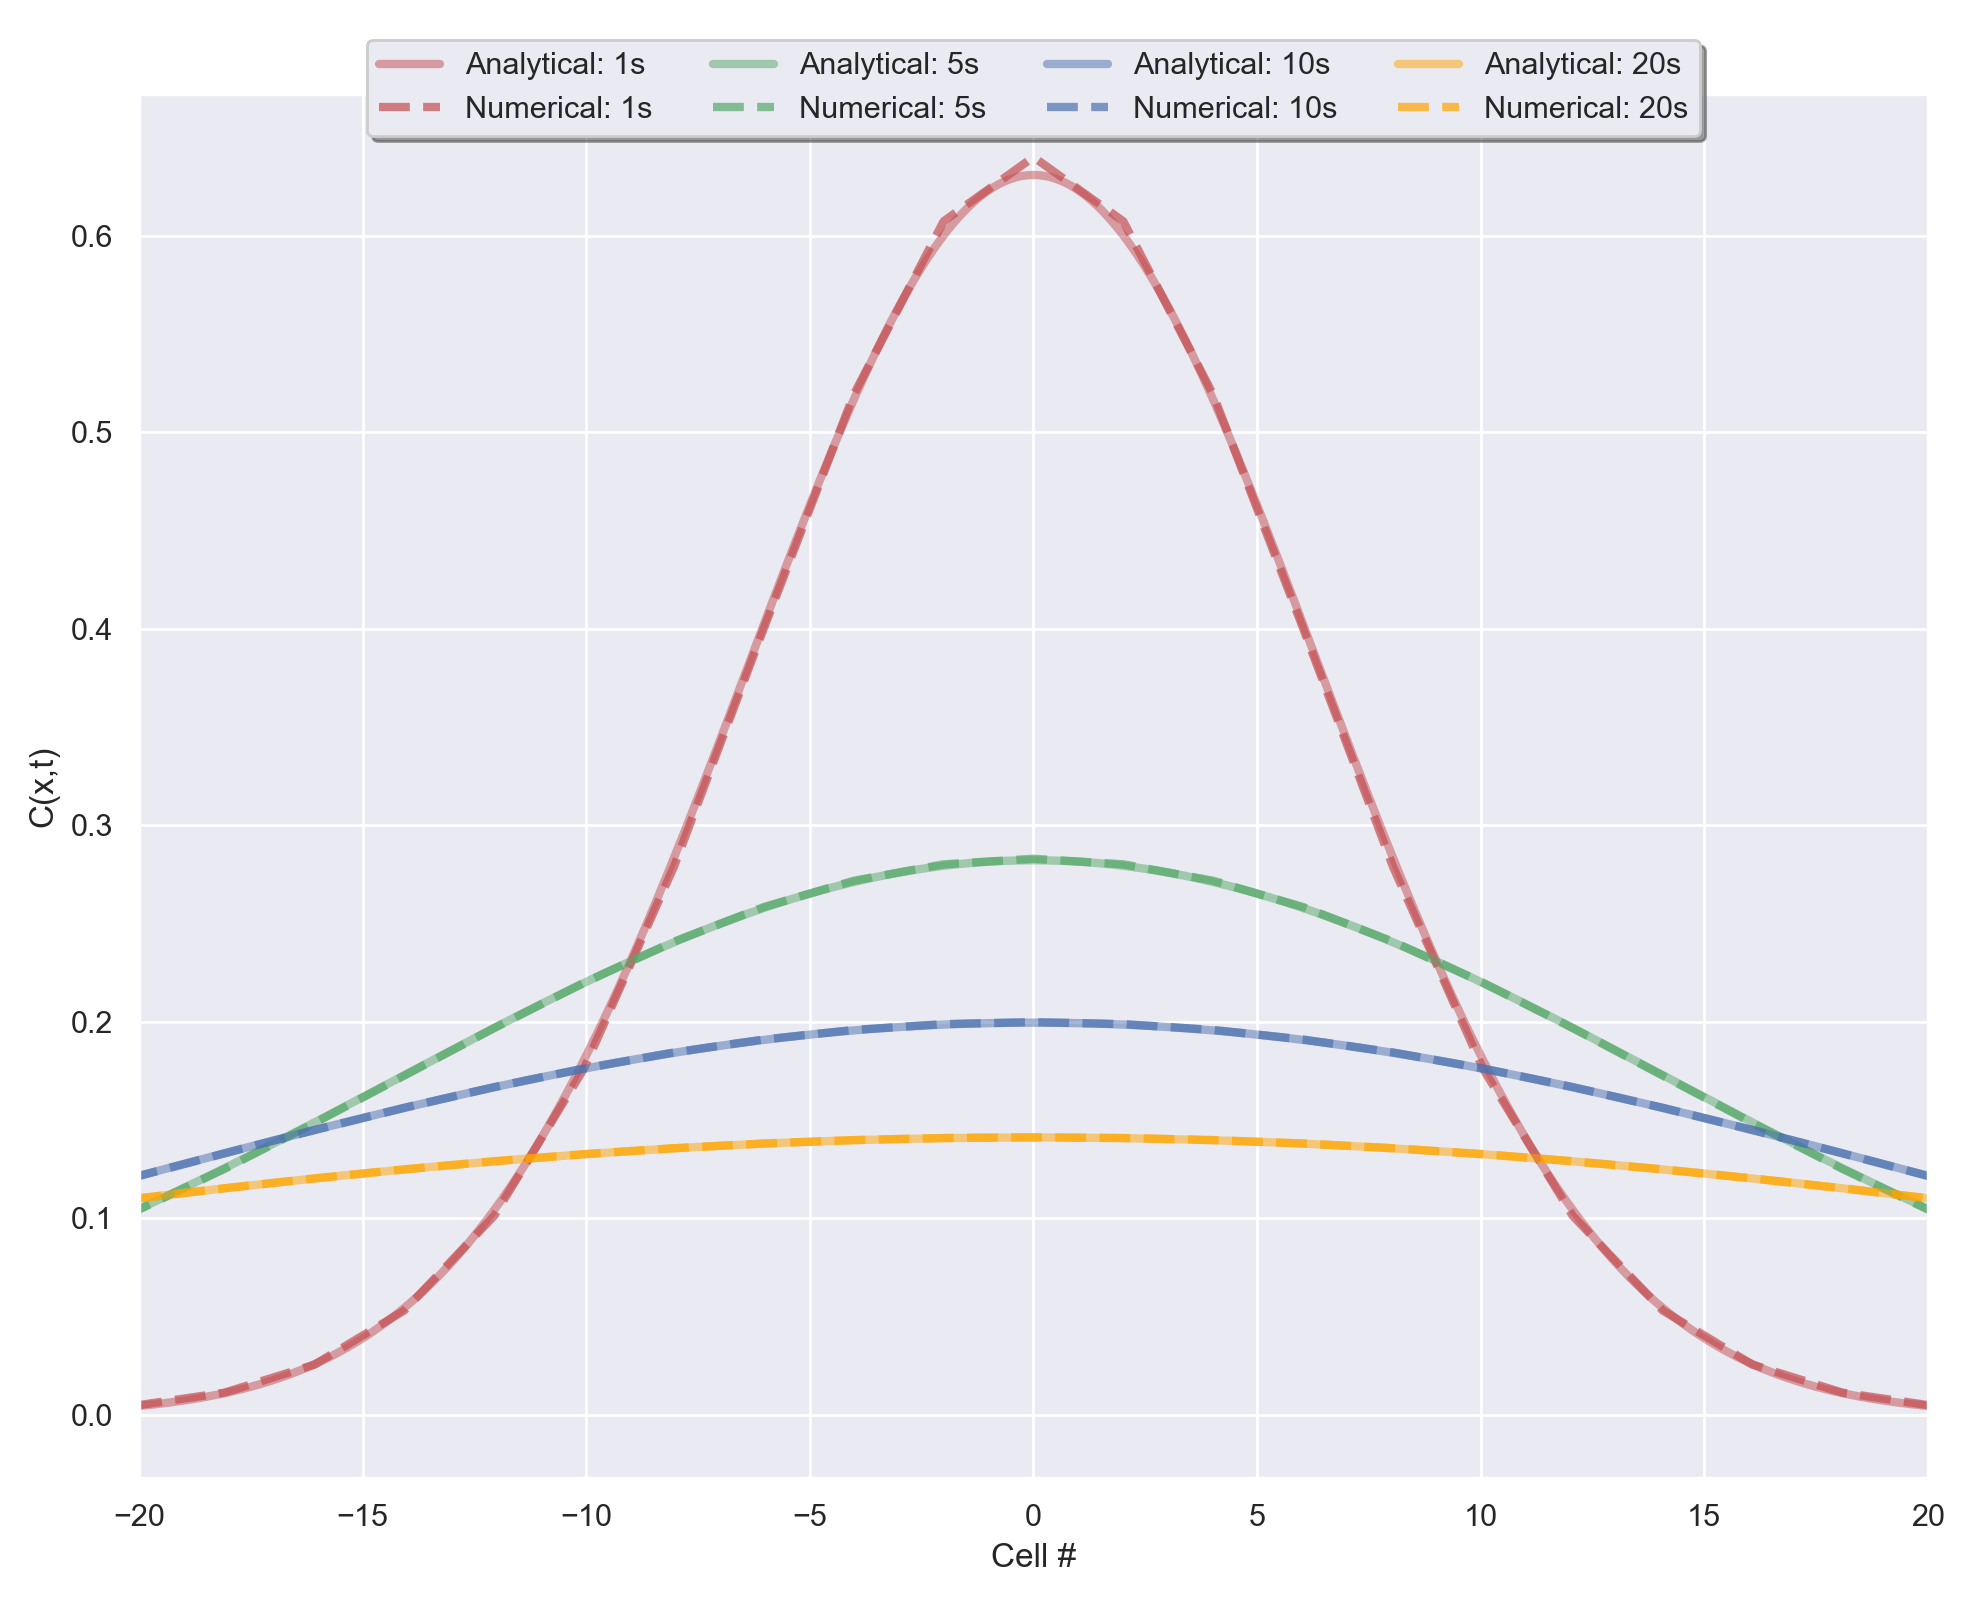
\includegraphics[width=\columnwidth]{figures/compare_equations.png}
  \caption{\label{fig:analyticalsolutions} Verification}
\end{figure}


\section{Results}


\subsection{Sensitivity analysis on effective diffusion shows importance of cell
  wall permeability}



\begin{figure}[!ht]
     \subfloat[First sub-figure\label{subfig-1:SAanalysis}]{%
       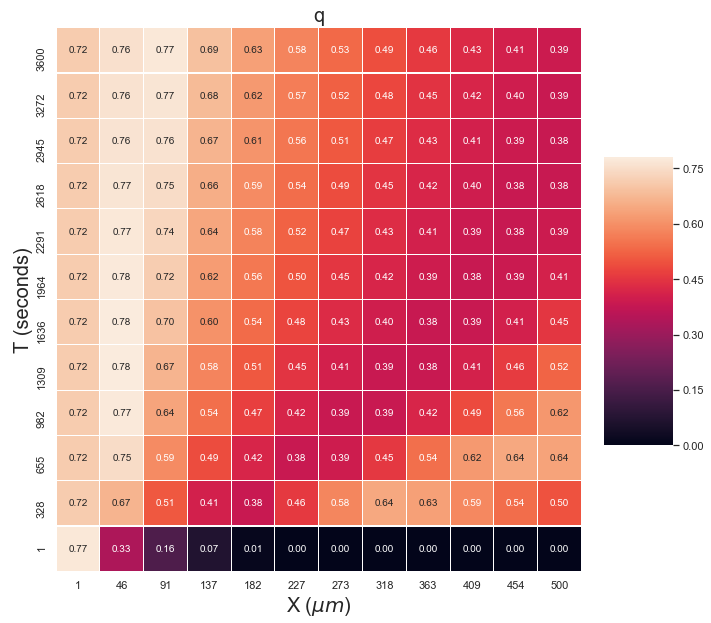
\includegraphics[width=0.5\columnwidth]{./figures/sa_matrix_first_order_q.png}
     }
     \subfloat[First sub-figure\label{subfig-2:SAanalysis}]{%
       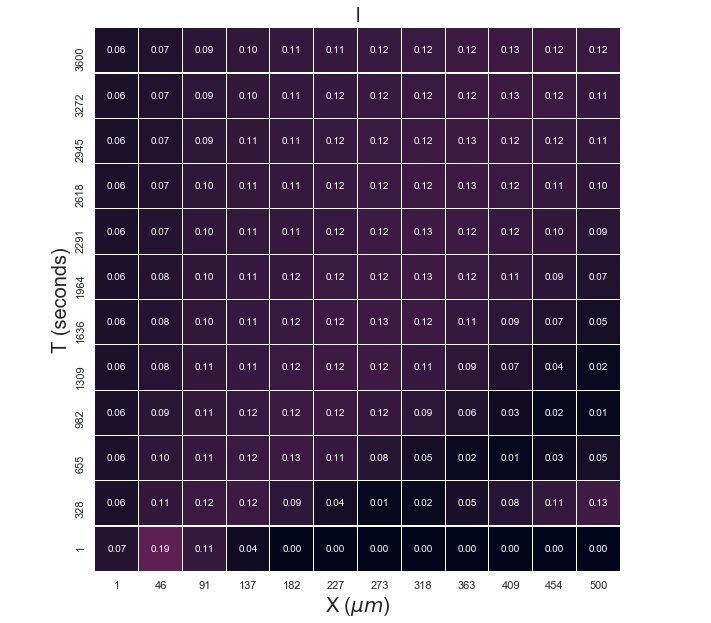
\includegraphics[width=0.5\columnwidth]{./figures/sa_matrix_first_order_l.png}
     }\\

     \subfloat[First sub-figure\label{subfig-3:SAanalysis}]{%
       \includegraphics[width=0.5\columnwidth]{./figures/sa_matrix_first_order_D.png}
     }
    
     \caption{Sobol analysis}
     \label{fig:SAanalysis}
   \end{figure}



\subsection{Changes to cell wall permeability explain flux reduction between cells}
\label{sec:cellwallperm}

\begin{figure}[ht]
  \centering
  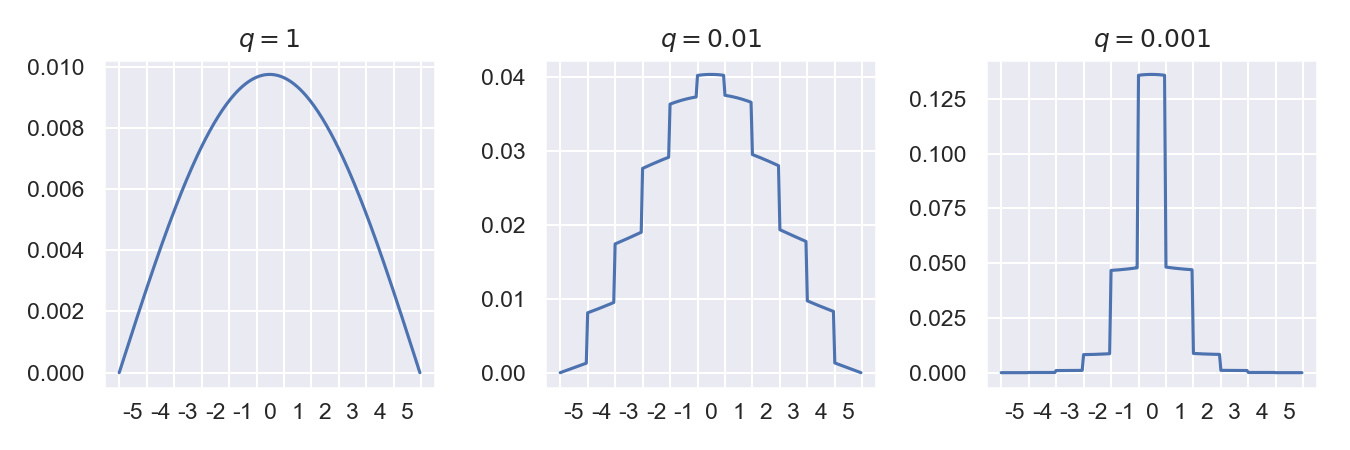
\includegraphics[width=\columnwidth]{figures/Waterfall.png}
  \caption{\label{fig:waterfall} Waterfall}
\end{figure}


\section{Conclusions}
This is useful because... 



\end{document}


%%% Local Variables:
%%% mode: latex
%%% TeX-master: "../main"
%%% End:
